\section{Isotropic elasticity}

We consider linear elasticity, i.e. using the generalized Hook's law:
\begin{equation}
 \CT: = \lambda \delta_{ij} \delta_{kl}+2\mu\delta_{ik} \delta_{jl}
  \label{eq:hook}
\end{equation}
where $\delta$ is the Kronecker delta, $\mu$ is the shear modulus,  $\lambda=2\mu\nu/(1-2\nu)$ is the so called
 Lam\'e constant with Poisson ratio $\nu$.
 
The elastic deformation is a reversible process. The related material behaviour is called elasticity. The Hooke's linear elastic law (Eqns. \ref{eq32} to \ref{eq34}) describes the elastic behaviour of solids. The elastic strain $\varepsilon$ is directly proportional to the effective stress $\sigma$.
\begin{eqnarray}
\varepsilon_x & = & \frac{1}{E}\cdot
\left(
\sigma_x\,-\,\nu\cdot
\left(
\sigma_y\,+\,\sigma_z
\right)
\right)
\label{eq32} \\[1.5ex]
\varepsilon_y & = & \frac{1}{E}\cdot
\left(
\sigma_y\,-\,\nu\cdot
\left(
\sigma_x\,+\,\sigma_z
\right)
\right)
\label{eq33} \\[1.5ex]
\varepsilon_z & = & \frac{1}{E}\cdot
\left(
\sigma_z\,-\,\nu\cdot
\left(
\sigma_x\,+\,\sigma_y
\right)
\right)
\label{eq34}
\end{eqnarray}

{\small
with
\begin{itemize}
\item[$\varepsilon_i$] -- strains,
\item[$\sigma_i$] -- stresses in Pa,
\item[$E$] -- Young's modulus in Pa,
\item[$\nu$] -- Poisson's ratio.
\end{itemize}
}
The Poisson's number $\mu$ can be derived by the following relation.
\begin{displaymath}
\mu\,=\,-\frac{\varepsilon_x}{\varepsilon_x}\,=\,-\nu
\end{displaymath}


 The following examples are utilized to verify
 the functionality of the software dealing with elastic deformation problems.

\subsection{Plane strain with uniform loading (2D)}
\subsubsection*{Problem definition}
\label{sec:el2d}
This example deals with calculations of a part of the whole rock mass.
This can be done when there are special conditions concerning symmetry,
structure of the rock mass and material behaviour.
To simulate an initial state of stress in different depths,
a pressure at least at one boundary has to be put on which represents
the load of the overburden. In addition to this the stresses decrease with
depth because of the gravity and the density of the rock mass (Fig. \ref{fme:cfound}).

\begin{figure}[!htb]
  \begin{center}
    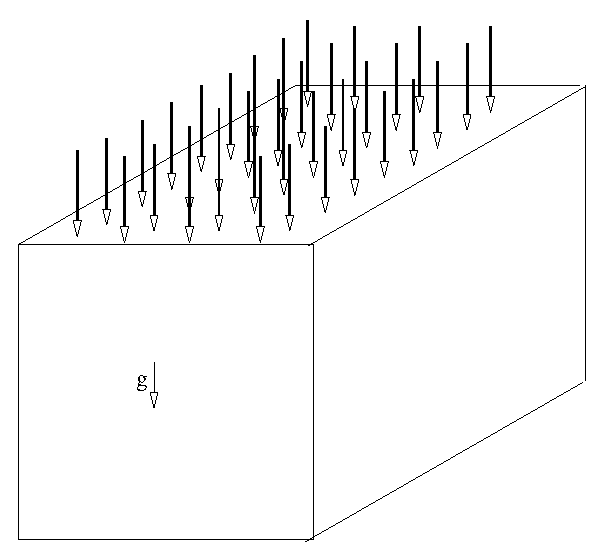
\includegraphics[scale=0.5]{M/ex_plate_model.eps}
  \end{center}
  \caption{Conceptual model of elastic foundation}
  \label{fme:cfound}
\end{figure}

The calculation area has a size of  $50m\times50m$ (length and height)
and the problem is simplified under the condition of plane strain.
The quadrilateral mesh is illustrated in Fig. \ref{fme:block},
   one corner of which is finely meshed in order that it can be used directly to
   conduct an elastic excavation simulation in a coming example.
\begin{figure}[!htb]
  \begin{center}
    \includegraphics[scale=0.3]{M/e1_mesh.eps}
  \end{center}
  \caption{Special discretization: 1150 quadrilateral elements, 1101 nodes }
  \label{fme:block}
\end{figure}
\subsubsection*{Initial and boundary conditions}
Initial conditions are not required for this problem. As for boundary conditions,
the top boundary is prescribed with a uniformly distributed pressure of $23.75MPa$. Such kind of boundary conditions
 are so called  traction boundary in the context of mechanics, they are treated as Neumann type boundary condition. More detailed boundary conditions are illustrated in Fig. \ref{fme:e1bc}.
\begin{figure}[!hbt]
  \centering
  \input{M/e1.eepic}
  \caption{Boundary conditions}
  \label{fme:e1bc}
\end{figure}
%

\subsubsection*{Material properties}
Homogeneous material properties are assumed within the whole domain. Table \ref{tme:el2d} gives the parameters.
 \begin{table}[!htb]
\centering
\begin{tabular}{lll}
\hline\hline\noalign{\smallskip}
Property & Value & Unit \\
\noalign{\smallskip}\hline\noalign{\smallskip}
Young's modulus & $25$  &GPa \\
Poisson's ratio & $0.3$             & $-$ \\
Density & $2500$             & $kg/m^3$ \\
\noalign{\smallskip}\hline\hline
\end{tabular}
\caption{Material parameters}
\label{tme:el2d}
\end{table}
%
\subsubsection*{Results}
For this simple elastic problem, we have an analytic solution given by
\begin{equation}
 \stress_{yy} = -23.75-\dens h\, \mbox[MPa]
  \label{eq:ex1_ana}
\end{equation}
where $\dens$ is the solid density and $h$ is the height from top to bottom boundary.


Fig. \mbox{\ref{fme:e1_syy} (left)} shows the distribution of vertical stress in the domain, which implies that the
 discretization error is very small. Fig. \mbox{\ref{fme:e1_syy} (right)} shows a linear variation of
   stress $\stress_{yy}$ along with height.
\begin{figure}[!thb]
  \begin{center}
  \epsfig{figure=M/e1_uy.eps,width=6cm, height=6cm}
  \epsfig{figure=M/ex1_plate_profile.eps,width=6cm, height=6cm}
  \end{center}
  \caption{Result of vertical stress, $\stress_{yy}$ (MPa). Left: domain distribution. Right: Vertical profile }
  \label{fme:e1_syy}
\end{figure}

The numerical result of $\stress_{yy}$ at the bottom boundary is \mbox{-24.97MPa}, which is very close to
 the analytic solution, $\stress_{yy}=-25.0\mbox{MPa}$. This proves the correction of the numerical scheme.


%
\subsubsection*{Benchmark deposit}
\begin{tabular}{|l|l|l|}
  \hline
  Benchmark & Problem type & Path in benchmark deposit \\
  \hline
 \emph{m\_drift} & M & benchmarks\verb \M\ \\
  \hline
\end{tabular}


%%initial stress state: given (directions), function (depth
%%dependent), isotropic (Poisson ratio 0.5)
%%
\newpage

\subsection[Excavation in homogeneous media (2D)]{Plain strain with uniform loading - Excavation in homogeneous media (2D)}
\label{sec:e2}
\subsubsection*{Problem definition}
This is the second step of the simulation described in the above
section, Section \ref{sec:el2d}. A long round tunnel is built in the rock mass and this is depicted in Fig. \ref{fme:excav}.
 The deformation due to the excavation  is simulated under the assumption of plane strain, same initial condition and materail parametrers given in Section {sec:el2d}.
\begin{figure}[!thb]
  \begin{center}
  \epsfig{figure=M/ex_plate.eps,width=7cm, height=7cm}
  \end{center}
  \caption{Excavation in rock mass }
  \label{fme:excav}
\end{figure}


\subsubsection*{Initial and boundary conditions}
The tunnel has a radius of $5m$. The released loading apprach is applied to simulate the excavation.

\subsubsection*{Results}
We use the same mesh as given in the above section to conduct the similation.
Fig. \ref{fig:e2cont} shows the distribution of vertical
displacement and and stresses in the domain after excavation.

\begin{figure}[!htb]
  \begin{center}
   %%\vspace{-2.7cm}
   \begin{minipage}[t]{0.45\textwidth}
     \begin{center}
    \includegraphics[scale=0.3]{M/ee_uy.eps}
    \centerline{Vertical displacement (m)}
    \end{center}
   \end{minipage}
  \hspace{0.02\textwidth}
   \begin{minipage}[t]{0.45\textwidth}
    \begin{center}
    \includegraphics[scale=0.3]{M/ee_sxx.eps}\\
    \centerline{Horizontal stress (MPa)}
    \end{center}
   \end{minipage}\\
  \end{center}
  \caption{State variables after excavation}
  \label{fig_modelhm}
\end{figure}

\begin{figure}[!htb]
  \begin{center}
   %%\vspace{-2.7cm}
   \begin{minipage}[t]{0.45\textwidth}
     \begin{center}
    \includegraphics[scale=0.3]{M/ee_sxy.eps}
    \centerline{Shear stress (MPa)}
    \end{center}
   \end{minipage}
  \hspace{0.02\textwidth}
   \begin{minipage}[t]{0.45\textwidth}
    \begin{center}
    \includegraphics[scale=0.3]{M/ee_syy.eps}\\
    \centerline{Vertical stress (MPa)}
    \end{center}
   \end{minipage}\\
  \end{center}
  \caption{State variables after excavation}
  \label{fig:e2cont}
\end{figure}
\subsubsection*{Benchmark deposit}
\begin{tabular}{|l|l|l|}
  \hline
  Benchmark & Problem type & Path in benchmark deposit \\
  \hline
 \emph{m\_drift} & M & benchmarks\verb \M\ \\
  \hline
\end{tabular}

\clearpage

\subsection[Excavation in heterogeneous media (2D)]{Plain strain with uniform loading - Excavation in heterogeneous media (2D)}
\label{sec:e3}
\subsubsection*{Problem definition}
Again, we analyze the deformation of the excavtion problem defined in Section \ref{sec:e2}. Contrary to homogeneous case,
  we  use function defined initial stress and assume four different material domains
 make up the geometry (Fig. \ref{fme:excav2}).
\begin{figure}[!thb]
  \begin{center}
  \epsfig{figure=M/m_drift_init.eps,width=7cm, height=7cm}
  \end{center}
  \caption{Excavation in heterogeneous rock mass }
  \label{fme:excav2}
\end{figure}


\subsubsection*{Initial and boundary conditions}
The initial stresses are assumed linearly distributed within a material domain.
 The expressions of these distribution are given in
 \begin{table}[!htb]
\centering
\begin{tabular}{llll}
\hline\hline\noalign{\smallskip}
Material & & Expression &  \\
  (Fig.  \ref{fme:excav2} ) &$\sigma_{xx}$ &$\sigma_{yy}$ &$\sigma_{zz}$  \\
\noalign{\smallskip}\hline\noalign{\smallskip}
   1 & $23.75+0.2y       $ &  $   23.75+0.2y     $   &  $     23.75+0.2y    $  \\
   2  & $24.75+0.5y       $ &  $   24.75+1.3y     $   &  $     24.75+0.5y    $ \\
   3  & $26.75+10.0x+12.0y  $ &  $  26.75+20.0x+16.0y $   &  $    26.75+10.0x+12.0y$  \\
   4  & $27.75+10.0x+14.0y $ &  $  27.75+20.0x+18.0y$   &  $   27.75+10.0x+14.0y$  \\
\noalign{\smallskip}\hline
\end{tabular}
\caption{Initial stress expression ( negative value, kPa)}
\label{tab:initialStress}
\end{table}

\subsubsection*{Material properties}
As depicted in Fig. \ref{fme:excav2}, the domain  consists of four different materials denoted
    by 1, 2, 3 and 4. Hereby, we assume only Young's modulus differs from each other of materials
    (Table \ref{tme:el2dHR}).
 \begin{table}[!htb]
\centering
\begin{tabular}{lll}
\hline\hline\noalign{\smallskip}
Property & Value & Unit \\
\noalign{\smallskip}\hline\noalign{\smallskip}
Young's modulus & {\color{red}1:}$25$, {\color{red}2:}26.0, {\color{red}3:}30.0,
   {\color{red}4:}28.0  &GPa \\
Poisson's ratio & $0.3$             & $-$ \\
Density & $2.5$             & $kg/m^3$ \\
\noalign{\smallskip}\hline\hline
\end{tabular}
\caption{Parameters}
\label{tme:el2dHR}
\end{table}

\subsubsection*{Results}

Fig. \ref{fme:exH_disp} shows the distribution of displacements after excavation.
 \begin{figure}[!thb]
  \begin{center}
  \epsfig{figure=M/ex_h_ux.eps,width=6cm, height=6cm}
  \epsfig{figure=M/ex_h_uy.eps,width=6cm, height=6cm}
  \end{center}
  \caption{Distribution of displacement (m)}
  \label{fme:exH_disp}
\end{figure}

\clearpage

Fig. \ref{fme:exH_stress} shows the distribution of stresses after excavation.
 \begin{figure}[!thb]
  \begin{center}
  \epsfig{figure=M/ex_h_sxx.eps,width=6cm, height=6cm}
  \epsfig{figure=M/ex_h_sxy.eps,width=6cm, height=6cm}
  \epsfig{figure=M/ex_h_syy.eps,width=6cm, height=6cm}
  \epsfig{figure=M/ex_h_szz.eps,width=6cm, height=6cm}
  \end{center}
  \caption{Distribution of stresses (kPa)}
  \label{fme:exH_stress}
\end{figure}

\subsubsection*{Benchmark deposit}
\begin{tabular}{|l|l|l|}
  \hline
  Benchmark & Problem type & Path in benchmark deposit \\
  \hline
 \emph{m\_drift\_init} & M & benchmarks\verb \M\ \\
  \hline
\end{tabular}
%%\subsubsection{Multiple excavation}

\clearpage

\subsection{Elastic cube (3D)}
\subsubsection*{Problem definition}
We consider deformation in a cubic domain under linearly distributed pressure (Fig. \ref{fig:brick}).
The size the domain is $1m\times1m\times1m$. The deformation is assumed being elastic.
\begin{figure}[!htb]
  \begin{center}
    \includegraphics[scale=0.3]{M/brick_l.eps}
  \end{center}
  \caption{A block with linear distributed pressure on the top surface}
  \label{fig:brick}
\end{figure}
\subsubsection*{Initial and boundary conditions}
 Normal translation on the vertical surfaces, which contains vertex A, D and
which contains vertex B, C, and on the bottom surface is restricted. On the top surface, a linear distributed
 pressure is prescribed in the manner of point-wise as:
 \begin{itemize}
   \item Vertex A: $1.0Pa$
   \item Vertex B:  $1.0Pa$
   \item Vertex C:  $0.0Pa$
   \item Vertex D:  $0.0Pa$
 \end{itemize}
The pressure at any point on the top surface is obtained by a linear interpolation before face integration.
This is done by programm automatically.
\subsubsection*{Material properties}
The material properties are homogenous with the domain and they are listed in Table \ref{tab:ecub}
 \begin{table}[!htb]
\centering
\begin{tabular}{lll}
\hline\hline\noalign{\smallskip}
Property & Value & Unit \\
\noalign{\smallskip}\hline\noalign{\smallskip}
Young's modulus & $2.0\times 10^{7}$  &Pa \\
Poisson's ratio & $0.4$             & $-$ \\
\noalign{\smallskip}\hline\hline
\end{tabular}
\caption{Material parameters of cubic domain}
\label{tab:ecub}
\end{table}
\subsubsection*{Results}
A deformed domain is depicted in Fig. \ref{fig:brick_d}, which demonstrated that the results
  are consistent with the prescribed boundary condition.
 \begin{figure}[!htb]
  \begin{center}
    \includegraphics[scale=0.4]{M/brick_l_d.eps}
  \end{center}
  \caption{Deformed cubic domain}
  \label{fig:brick_d}
\end{figure}
\subsubsection*{Benchmark deposit}
\begin{tabular}{|l|l|l|}
  \hline
  Benchmark & Problem type & Path in benchmark deposit \\
  \hline
 \emph{m\_brick\_l} & M & benchmarks\verb \M\ \\
  \hline
\end{tabular}

\clearpage

\subsection{Given deformation at the top (3D)}

\textbf{Problem definition}

A quarter of an elastic cylinder is compressed at the top. The deformation that is caused by a uniform vertical stress is given as boundary condition. The aim is to calculate the stress in $z$-direction which is caused by this deformation and to get to know the resulting deformations in each direction.

\begin{figure}[htbp]
\centering
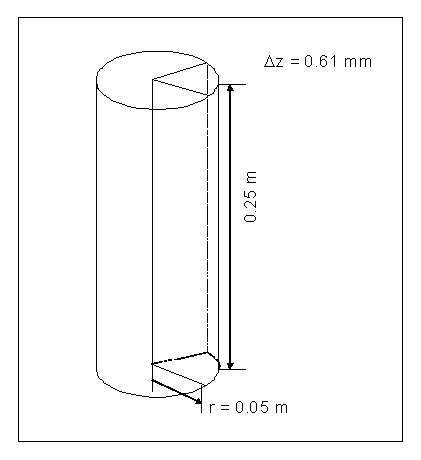
\includegraphics[width=0.4\textwidth]{M/figures/fig31.eps}
\caption{Calculation area: a quarter of a cylinder}
\label{fig31}
\end{figure}

%\newpage

\textsl{Assumptions}

\begin{tabbing}
\=xxxxxxxxxx  \=xxxxxxxxxxxxxxxxxxxxxxx \kill
\> Solid: \> homogeneous, isotropic, finite dimensions, constant deformation, \\
\> \> linear elastic material behaviour
\end{tabbing}

\textbf{Model set-up of the 3D numerical model}

For the 3-dimensional simulation the calculation area is exclusively out of a quarter of a cylinder. The model includes 4000 elements and 4947 nodes. Deformations in $x$-direction are suppressed in the $y-z$-plane. Deformations in $y$-direction are suppressed in the $x-z$-plane and deformations in $z$-direction are inhibited at the bottom of the quarter cylinder. At the top of the model a mechanical boundary condition is set with a constant displacement of 0.61~mm. The elastic deformation of the solid is not time-dependent. The used material parameters are shown in Tab. \ref{tab33}.
\begin{table}[htbp]
\centering
\begin{tabular}{|c|l|l|}
\hline
symbol & quantity & value \\
\hline
$\rho$  & density of the solid &  2.5 t$\cdot$m$^{-3}$  \\			
\hline
$E$ & Young's modulus of the solid & 7 GPa \\
\hline
$\nu$ & Poisson ratio & 0.3 \\
\hline
\end{tabular}
\caption{Material parameters}
\label{tab33}
\end{table}

\begin{figure}[htbp]
\centering
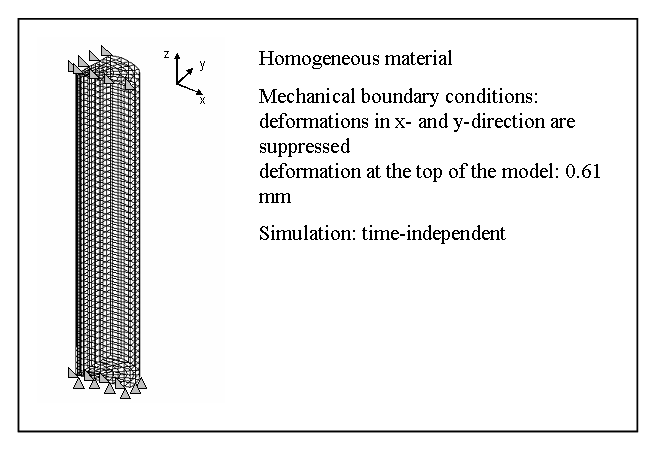
\includegraphics[width=0.5\textwidth]{M/figures/fig32.eps}
\caption{Calculation model (3D)}
\label{fig32}
\end{figure}

\newpage

\textbf{Evaluation method}

In order to solve the equations of the Hooke's law, there are some constraints that have to be considered: the stresses in $x$- and $y$-direction are equal to zero, because the body can expand into radial direction. Thus the Hooke's equations can be simplified as follows:
\begin{eqnarray}
\varepsilon_z & = &
\frac{\Delta z}{z}\,=\,\frac{1}{E}\cdot\sigma_z
\label{eq36} \\[1.5ex]
\varepsilon_x & = &
\varepsilon_x\,=\,\frac{1}{E}\cdot\left(-\nu\cdot\sigma_z\right)
\label{eq37}
\end{eqnarray}

\textbf{Results}

With the given strain in $z$-direction, the stress $\sigma_z$ is calculated by Eqn. \ref{eq36}.
\begin{displaymath}
\frac{\Delta z}{z}=\frac{-6.1\cdot 10^{-4}\,\mathrm{m}}{0.25\,\mathrm{m}}=-2.44\cdot 10^{-3}
\quad\mathrm{and}\quad
\sigma_z=-2.44\cdot 10^{-3}\cdot 7\cdot 10^{9}\,\mathrm{Pa}=
-1.71\cdot 10^{7}\,\mathrm{Pa}
\end{displaymath}

In this way, the strains in $x$- and $y$-direction are known.
\begin{displaymath}
\varepsilon_x\,=\,\varepsilon_y\,=\,
\frac{1}{7\cdot 10^{9}\,\mathrm{Pa}}\cdot
\left(-0.3\cdot-1.71\cdot 10^{7}\,\mathrm{Pa}\right)\,=\,
7.32\cdot 10^{-4}
\end{displaymath}

The numerical results meet exactly the analytical solutions. This is sketched in Fig. \ref{fig33}, where the strains and the resulting stress along a polyline from top to bottom of the quarter cylinder can be found. That means both RockFlow and GeoSys/RockFlow are able to calculate the state of stresses for the 3D elastic deformation.

\clearpage

\begin{figure}[htbp]
\centering
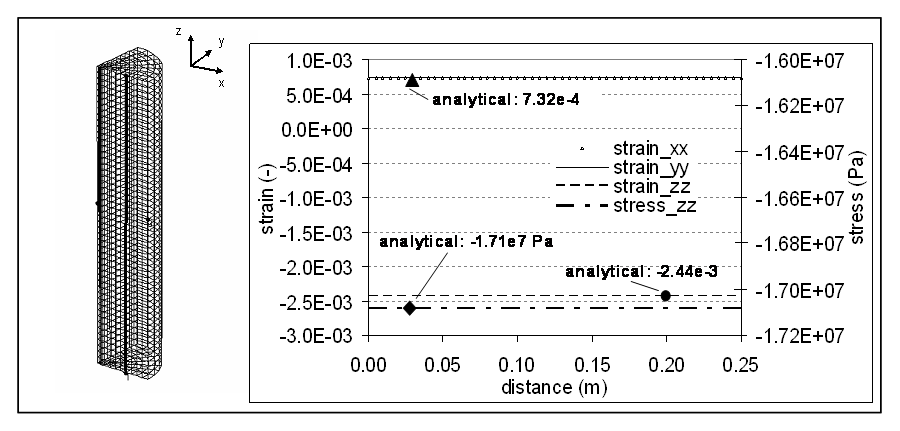
\includegraphics[width=0.9\textwidth]{M/figures/fig33.eps}
\caption{Strains and stress in $z$-direction as the result of deformation}
\label{fig33}
\end{figure}

\vskip 4.0ex

\begin{tabular}{|l|l|l|l|}
\hline
Path in the & Used code	& Used version & Date of si- \\
benchmark deposit	& & & mulation run \\
\hline	
$\backslash$M$\backslash$elastic\_deformation$\backslash$	& GeoSys/RockFlow	& RockFlow 4,	& Dec. 2007 \\
displacement$\backslash$displ\_Geosys/	& & rf4-507 & \\
RF$\backslash$m\_e\_displacement\_3Du	& & & \\
\hline	
\end{tabular}


\clearpage

\subsection{Given stress at the top (3D)}

\textbf{Problem definition}

This example is the inverse of the precedent one. The quarter cylinder is deformed by a given stress, while this time the resulting deformation is unknown. In order to check out easily whether the simulated results correspond to the analytical solutions, the value of the effective stress in $z$-direction on top of the calculation model is the same as in the above described example.

\textsl{Assumptions}

\begin{tabbing}
\=xxxxxxxxxx  \=xxxxxxxxxxxxxxxxxxxxxxx \kill
\> Solid: \> homogeneous, isotropic, finite dimensions, constant deformation, \\
\> \> linear elastic material behaviour
\end{tabbing}

\textbf{Model set-up of the 3D numerical model}

The calculation model has the same properties as the model of the precedent example. At the top of the model a load of -1.71$\cdot$10$^7$~Pa was set as constant source term. The simulation with both RockFlow and Geosys/RockFlow needs the input of the load as source term in $z$-direction at the single nodes under consideration of each element node. The input is done as single forces, not as the common stresses. The displacement boundaries are the same as in the precedent example except the $z$-displacement on the top of the model. The used material parameters are shown in Tab. \ref{tab33}.

%\newpage

\textbf{Results}

The analytical solution and results are identical to the previous example. The calculated displacement as a result of the constant load on the top amounts to 6.1$\cdot$10$^{-4}$~m. The numerical results that are shown in Fig. \ref{fig34} meet the analytical solutions well.

\begin{figure}[htbp]
\centering
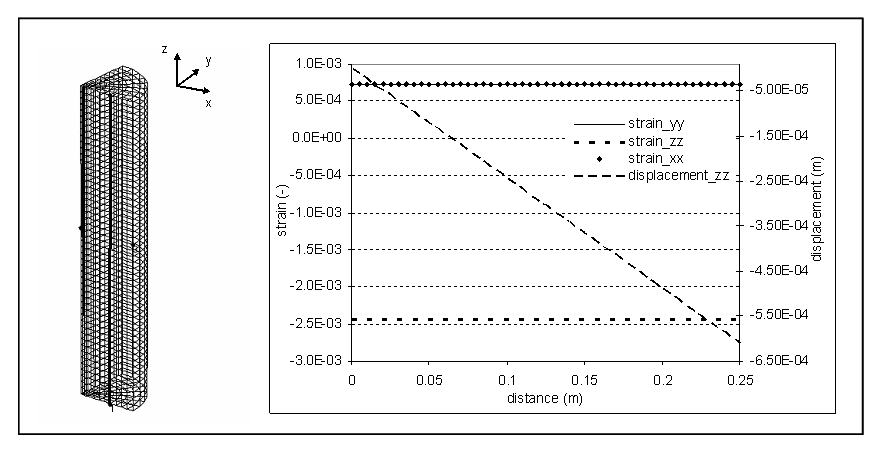
\includegraphics[width=0.9\textwidth]{M/figures/fig34.eps}
\caption{Strains and displacement in $z$-direction}
\label{fig34}
\end{figure}

\begin{tabular}{|l|l|l|l|}
\hline
Path in the & Used code	& Used version & Date of si- \\
benchmark deposit	& & & mulation run \\
\hline
$\backslash$M$\backslash$elastic\_deformation$\backslash$	& GeoSys/RockFlow	& RockFlow 4,	& Dec. 2007 \\
stress$\backslash$stress\_Geosys/RF$\backslash$	& & rf4-507 & \\
m\_e\_stress\_3Du	& & & \\
\hline	
\end{tabular}


\clearpage

\subsection{Lubby1: Nonlinear model}
\label{subsec:lubby1}
The Lam{\'{e}} constants defined for Hooke's fourth-order elastic material tensor (\ref{eq:hook}) can be expressed by the Young's modulus $E$, the Poisson's ratio $\nu$ and the shear modulus $G$ (so-called {\sl enginering constants}) which can be obtained experimentally.
\begin{eqnarray}
\mu     & = & \ttfrac{E}{2(1+\nu)}\,=\,G \\[1.5ex]
\lambda & = & \ttfrac{E\nu}{(1+\nu)(1-2\nu)}\,=\,\ttfrac{2G\nu}{(1-2\nu)}
\end{eqnarray}

In many technical applications considering small strains, the elastic material parameters are assumed to be constant, and the stress-strain curves are nearly linear. However, the typical response of certain geological materials to monotonic loading (without load reversal) shows a nonlinear stress-strain behavior. Considering only elastic effects during load application, Hooke's law cannot be used to describe the observed material properties. Therefore, so-called pseudo-elastic constitutive models are frequently used for the analysis of nonlinear stress-strain curves, particularly in soil and rock mechanics. In a generalized manner, they are based on the assumption of an explicit stress-strain relation considering a stress- and strain-dependent material matrix:
\begin{equation}
\mio{\sigma}{}{}\,=\,\fourtens{\mathcal{C}}(\mio{\sigma}{}{},\mio{\varepsilon}{}{})\ccdot\mio{\varepsilon}{\mathrm{e}}{}\,.
\label{elasticity_nonlin}
\end{equation}

Based on the so-called {\sl Lubby1} model (cf. \cite{Lux:1984}), a nonlinear elastic approach with strain-dependent Young's modulus
\begin{equation}
E(\varepsilon_{\mathrm{v}})\,=\,\frac{E_0}{1+a\,\varepsilon_{\mathrm{v}}^n}
\label{lubby1_ev}
\end{equation}
but constant Poisson's ratio is proposed. Here, $\varepsilon_{\mathrm{v}}$ is the equivalent strain, and $E_0$, $a$ as well as $n$ are material parameters . The equivalent strain is defined by
\begin{equation}
\varepsilon_{\mathrm{v}}\,=\,
\sqrt{\frac{2}{3}\,\mio{\varepsilon}{\mathrm{e}}{}\ccdot\mio{\varepsilon}{\mathrm{e}}{}}\,.
\end{equation}

\subsubsection*{Problem definition}

Triaxial short-term compression under axisymmetric conditions is carried out to verify the nonlinear elastic isotropic material model (modified Lubby1 approach). For the calculation, the cross-section of a cylindrical sample with a radius of 30~mm and a height of 120~mm is studied. The loading in principal axes includes a radial pressure as well as an axial displacement, and is realized in two steps. It is resulting in a homogeneous stress-strain state. Details of the model (geometry, mesh, boundary conditions) according to K.-H. Lux and F. Werunsky (unpublished report, 2008) are presented in Fig.~\ref{triax_model_lubby1}.

\begin{figure}[!htb]
\begin{center}
\includegraphics[width=0.2\textwidth]{M/figure/svv_model.eps}
\hspace*{10.0ex}
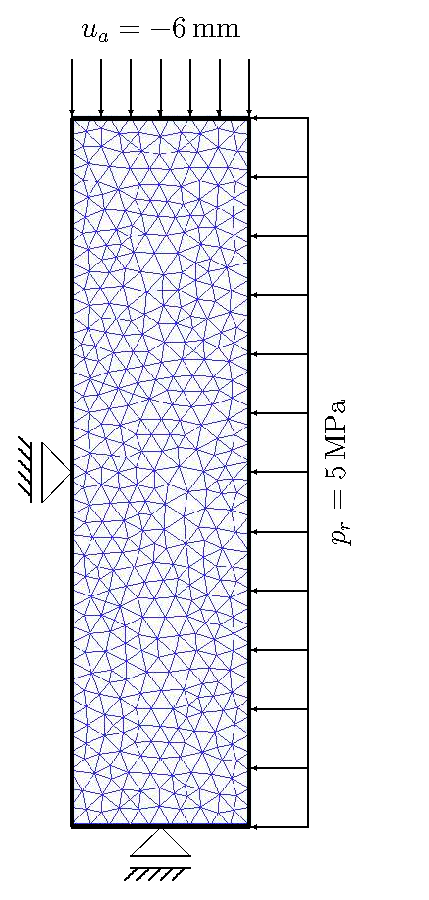
\includegraphics[width=0.25\textwidth]{M/figure/svv_mesh.eps}
\end{center}
\caption{Triaxial compression of a cylindrical sample. Axisymmetric model. Left: Geometry. Right: Finite element grid and boundary conditions.} 
\label{triax_model_lubby1}
\end{figure}

\begin{figure}[!htb]
\begin{center}
\includegraphics[width=0.6\textwidth]{M/figure/svv_loadhistory.eps}
\end{center}
\caption{Triaxial compression of a cylindrical sample. Loading history for short-term experiments. Radial casing pressure (stress rate $\dot{p}{}_r=0.25$\,MPa$\cdot$s$^{-1}$) with subsequent axial displacement (strain rate $\dot{\varepsilon}{}_a=3.47\cdot 10^{-5}$\,s$^{-1}$).} 
\label{triax_loadhist_lubby1}
\end{figure}

\subsubsection*{Initial and boundary conditions}

Initial conditions do not have to be given for the problem under consideration. As the bottom edge is fixed in vertical direction, the left-hand edge is fixed in horizontal direction for symmetry reasons (axis of rotation). On the right-hand edge initially a radial casing pressure of 5~MPa is applied within 20~seconds with a constant stress rate. While keeping constant this radial pressure, a subsequent stroke-driven axial compressive loading is applied within the following 1\,440~seconds with a constant strain rate. The maximum axial displacement is 6~mm which corresponds to a 5\% reduction of the sample's height (for the complex loading history cf. Fig.~\ref{triax_loadhist_lubby1}).

\subsubsection*{Material properties}
 
The material parameters referring to the modified Lubby1 relation~(\ref{lubby1_ev}) are summarized in Tab.~\ref{matpar_lubby1}. Within this context, the initial Young's modulus and the Poisson's ratio are close to values known for rock salt.
 
\vskip 3.0ex
 
\begin{table}[!htb]
\centering
\begin{tabular}{lll}
\hline\hline\noalign{\smallskip}
Property & Value & Unit \\
\noalign{\smallskip}\hline\noalign{\smallskip}
Poisson's ratio $\nu$             & 0.335   & --  \\
initial Young's modulus $E_0$     & 21\,400 & MPa \\
factor $a$ in (\ref{lubby1_ev})   & 2\,750  & --  \\
exponent $n$ in (\ref{lubby1_ev}) & 1.0     & --  \\
\noalign{\smallskip}\hline\hline
\end{tabular}
\caption{Material parameters}
\label{matpar_lubby1}
\end{table}

\subsubsection*{Results}

The representation of the axial stress vs. the axial strain in Fig.~\ref{triax_res_lubby1} shows on exemplarily chosen material parameters the noticeable difference between the linear (Hooke's model) and the nonlinear (modified Lubby1 model) elastic models even at small strains. Within the contect of the studied case, the stress response will be overestimated by a multiple using the linear Hooke's law. 

\clearpage

\begin{figure}[!htb]
\begin{center}
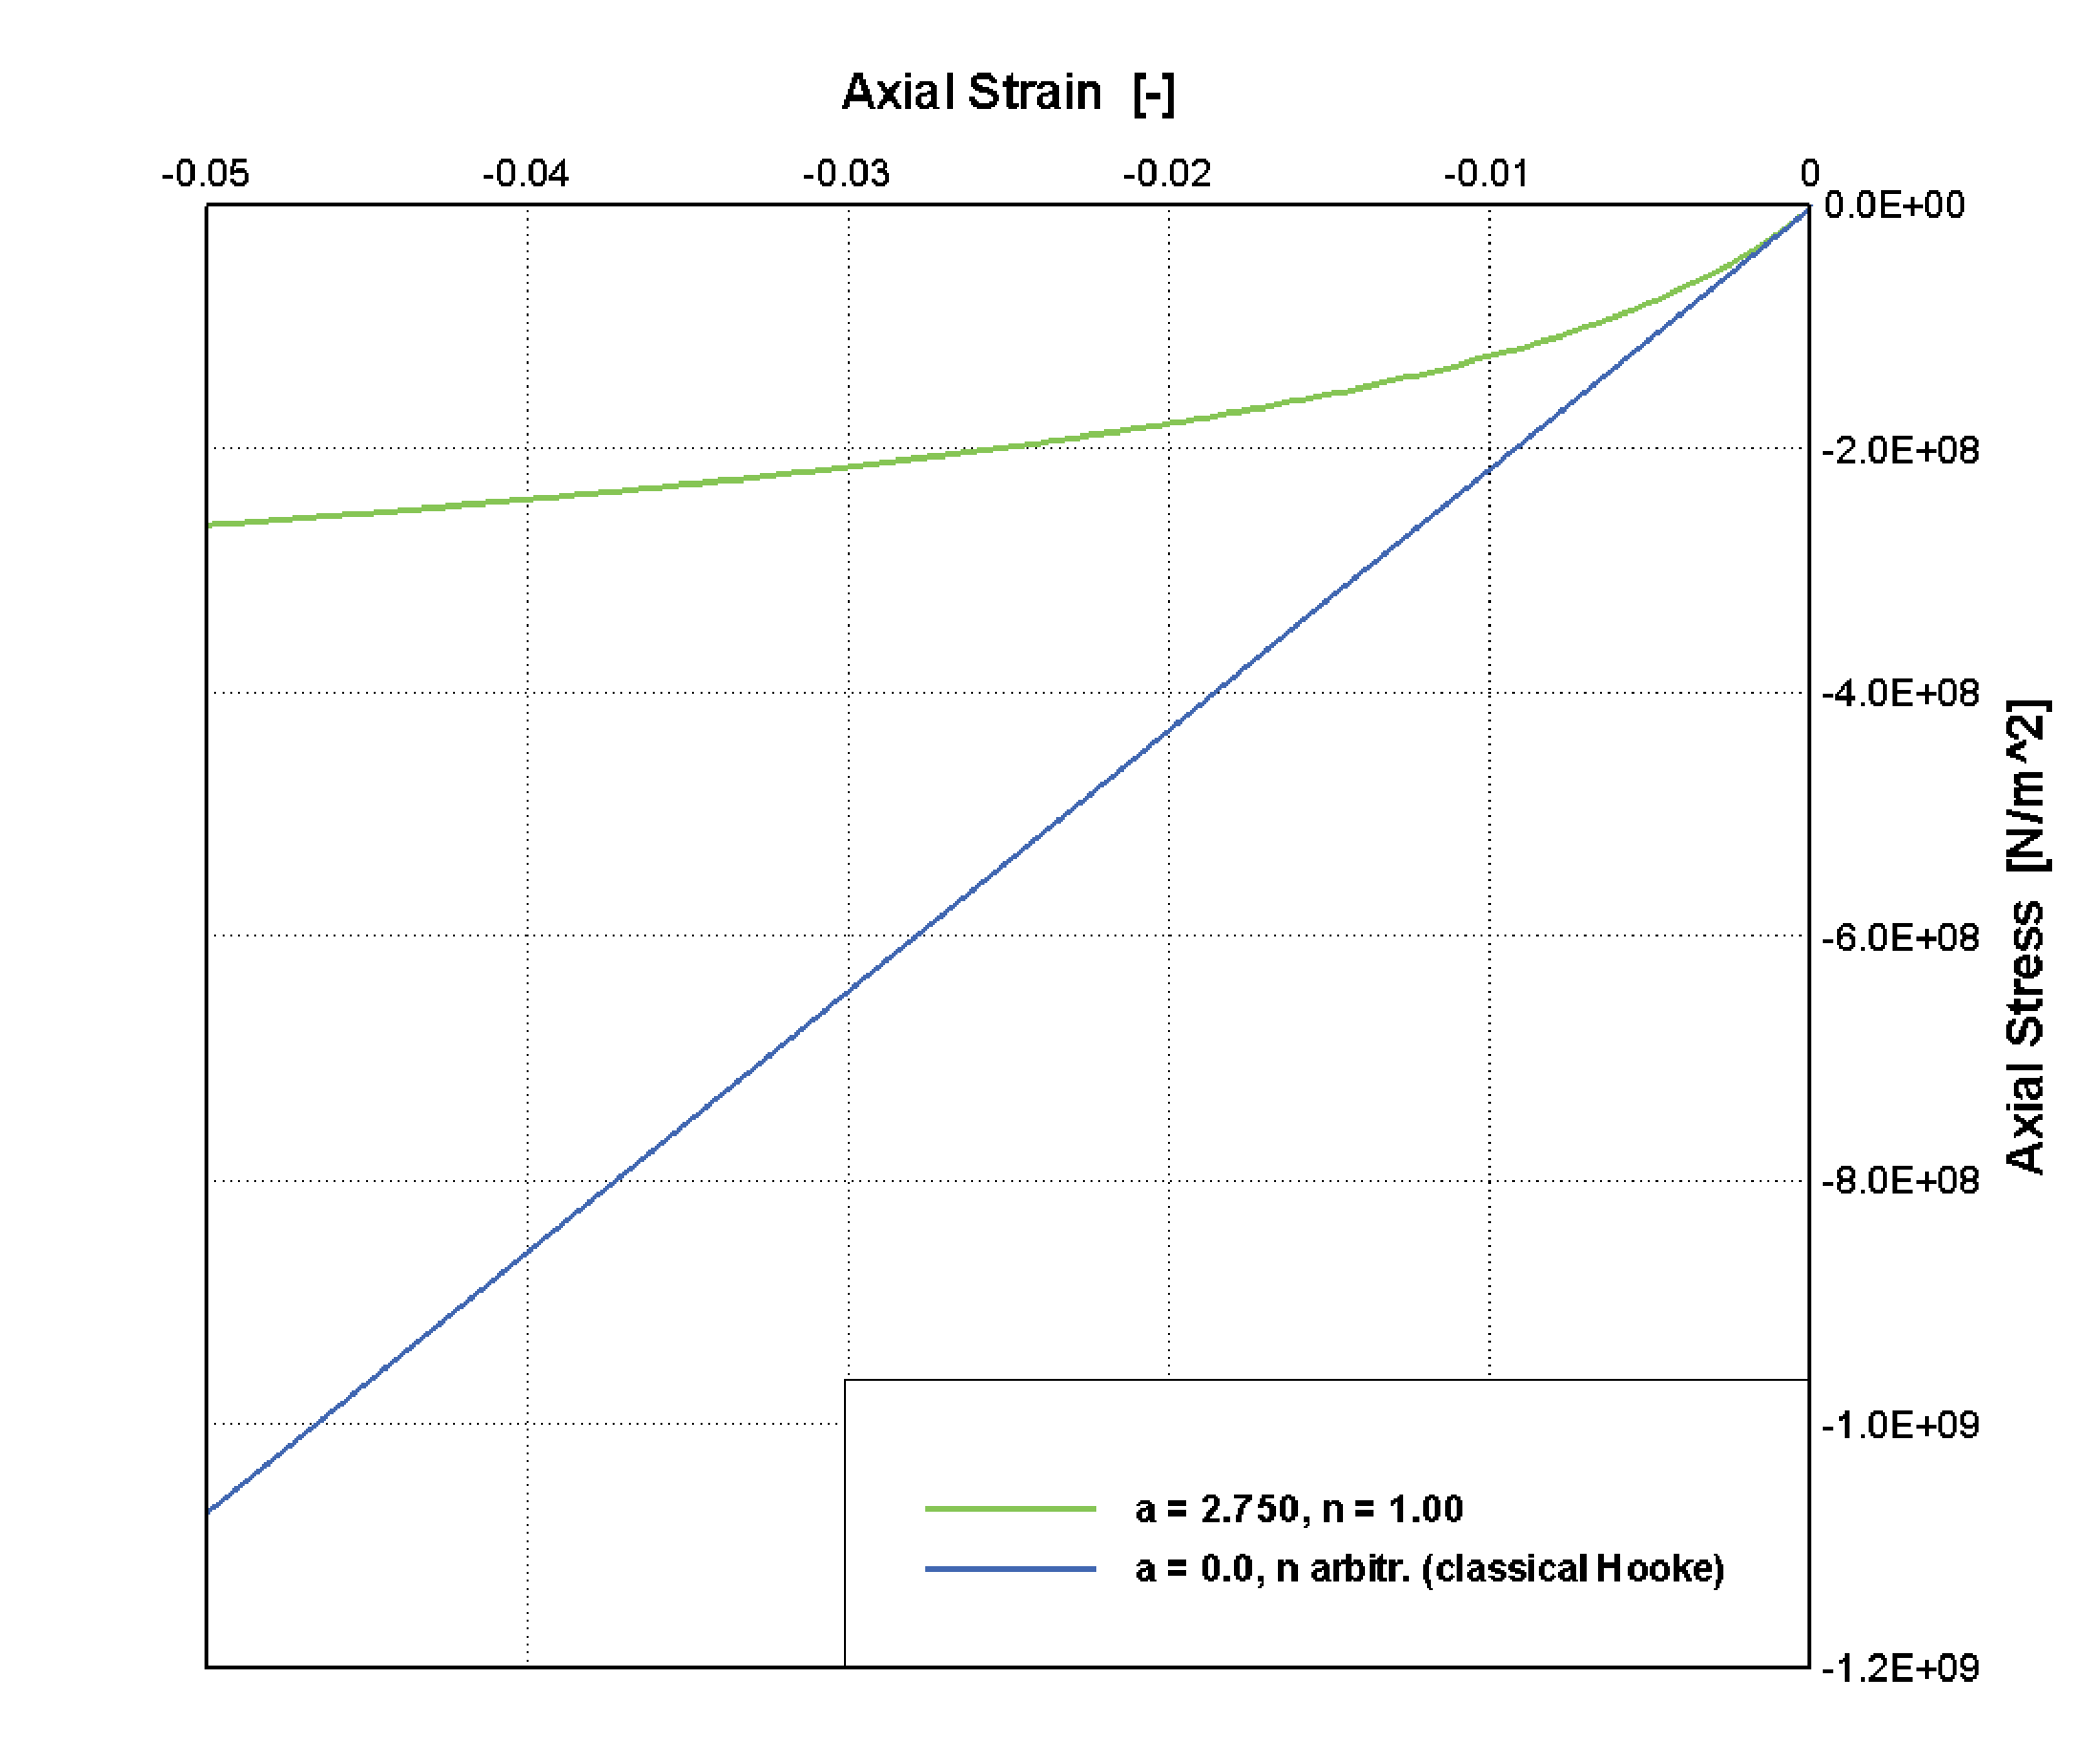
\includegraphics[width=0.6\textwidth]{M/figure/svv_e_stress_strain_hooke_lubby1m.eps}
\end{center}
\caption{Triaxial compression of a cylindrical sample. Stress-strain curves regarding the axial load response. Comparison of linear elastic (Hooke) and nonlinear elastic (modified Lubby1~(\ref{lubby1_ev})) material models.} 
\label{triax_res_lubby1}
\end{figure}

\vskip 4.0ex

\subsubsection*{Benchmark deposit}

\begin{tabular}{|l|l|l|}
  \hline
  Benchmark & Problem type & Path in benchmark deposit \\
  \hline
 \emph{m\_triax\_lubby1} & M & benchmarks\verb \M\ \\
  \hline
\end{tabular}



